\documentclass{beamer}
\usepackage{hyperref}
%\usepackage[utf8]{inputenc}
% \usepackage[T1]{fontenc}
\usepackage{amsmath,amssymb,amsfonts,textcomp,setspace,graphicx,tikz,color}
\usepackage[absolute,overlay]{textpos}
 \setlength{\TPHorizModule}{1mm}
 \setlength{\TPVertModule}{1mm}

\title{Integrative Omics Data Analysis, \\ Lights and Shadows}
\author{Alex S\'anchez--Pla}
\date{February 25, 2021}
\usetheme{Copenhagen}

\include{macros}


\begin{document}

\begin{frame}
	\begin{scriptsize}
		\begin{center}
			\emph{V Jornadas de Bioinform\'atica. Universidad de Granada}
		\end{center}
	\end{scriptsize}
	
	\titlepage
	
	\begin{columns}
	\column{0.7\textwidth}
	   \scriptsize
		Genetics, Microbiology \& Statistics\\
		\textbf{Facultad de Biología, Universitat de Barcelona}\\
		Statistics and Bioinformatics Unit (UEB)\\
		\textbf{Vall Hebron Institut de Recerca}
		
		\hfill\column{0.3\textwidth}
		\includegraphics[height=1.25cm]{images/alllogos.png}
		% \includegraphics[height=0.5cm]{images/VHIR_fonstransp.png}
		
	\end{columns}
\end{frame}


\frame<0>{
%\addtocounter{totalframenumber}{-1}
\titlepage
}

\begin{frame}%[Frame 1]
\addtocounter{framenumber}{-1}
\frametitle{Table of Contents}
\tableofcontents
\end{frame}


\section{Introduction and Background}

 
 \begin{frame}
 \begin{center}
{\huge 	Presentation and Objectives	}
 \end{center}
 \end{frame}
  
  \begin{frame}
  	\frametitle{Who, where, what?}
  	 \begin{figure}[ht]
  	 	\centering
  	 	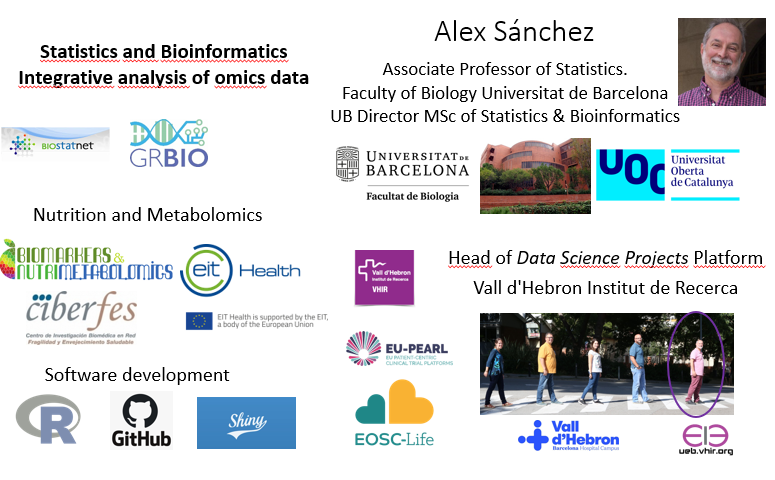
\includegraphics[width=100mm]{images/AlexSanchezPresentation.png}
  	 \end{figure}
  \end{frame}
 
 \begin{frame}
 	\frametitle{Multiversity teaching}
 	\begin{figure}[ht]
 		\centering
 		\includegraphics[width=100mm]{images/docenciaMultiversitaria.png}
 	\end{figure}
 \end{frame}

\begin{frame}
	\frametitle{The UOC-UB MSc in Bostatistics and Bioinformatics}
	\begin{figure}[ht]
		\centering
		\includegraphics[width=100mm]{images/MasterUOCGeneral.png}
	\end{figure}
\end{frame}
 
 
 \begin{frame}
 	\frametitle{The UOC-UB MSc in Bostatistics and Bioinformatics}
 	\begin{figure}[ht]
 		\centering
 		\includegraphics[width=100mm]{images/MasterUOCItinierary.png}
 	\end{figure}
 \end{frame}
 
 
 \subsection{From Biology to Omics and to Multi-Omics} 
  
  \begin{frame}
  \begin{center}
  	Omics, Omics Data \\ and Omics Integration 
  \end{center} 	
  \end{frame}
  
  \begin{frame}
  	\frametitle{What is ``omics''?}
  	\begin{itemize}
  		\item In biological context , the suffix ``omics'' is used to refer to the study of large sets of biological molecules (Smith et al., 2005)
  		\item The study of different components participating and/or regulating complex biological processes, triggered the development of several fields that, together, are described with the term OMICS.
  	\end{itemize}
  		\begin{figure}[ht]
  			\centering
  			\includegraphics[width=30mm]{images/Imagen5.jpg}
  		\end{figure} 
  \end{frame}
  
  
  \begin{frame}
  	\frametitle{The central dogma}
  	\begin{figure}[ht]
  		\centering
  		\includegraphics[width=45mm]{images/Imagen6.jpg}
  		\includegraphics[width=45mm]{images/Imagen0.jpg}
  	\end{figure} 
  \end{frame}
  
  
  \begin{frame}
  	\frametitle{The Omics Cascade (1): ``omes''}
  	\begin{figure}[ht]
  		\centering
  		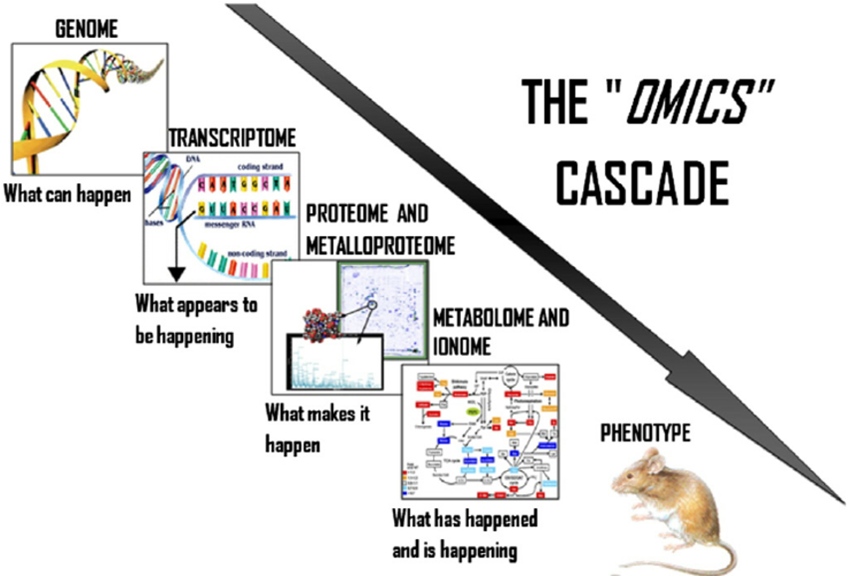
\includegraphics[width=80mm]{images/omicsCascade.png}
  	\end{figure} 
  \end{frame}
  
  
  \begin{frame}
  	\frametitle{We study omes with omics}
  	\begin{figure}[ht]
  		\centering
  		\includegraphics[width=100mm]{images/Imagen9.jpg}
  	\end{figure} 
  \end{frame}
  
  
\begin{frame}
  	\frametitle{Genomics}
  	\begin{columns}%
  		\begin{column}[t]{0.45\textwidth}%
  			Genomics is a discipline in genetics that applies recombinant DNA, DNA sequencing methods, and bioinformatics to sequence, assemble, and analyze the function and structure of genomes (the complete set of DNA within a single cell of an organism)
  		\end{column}
  		  		
  		\begin{column}[t]{0.45\textwidth}%
  			\begin{figure}[ht]
  				\centering
  				\includegraphics[width=50mm]{images/Imagen10.jpg}
  			\end{figure} 
  		\end{column}
  	\end{columns}
  \end{frame}



 \begin{frame}
 	\frametitle{Transcriptomics}
 	\begin{columns}%
 		\begin{column}[t]{0.45\textwidth}%
 			\begin{itemize}
 				\item The transcriptome is the set of all RNA molecules, in one or a population of cells.
 				\item Transcriptomics, examines expression levels of mRNAs in a given cell population, often using high-throughput techniques: microarrays or NGS.
 			\end{itemize}
 		\end{column}
 		
 		\begin{column}[t]{0.45\textwidth}%
 			\begin{figure}[ht]
 				\centering
 				\includegraphics[width=55mm]{images/Imagen11.jpg}
 			\end{figure} 
 		\end{column}
 	\end{columns}
 \end{frame}
 
 
 
 \begin{frame}
 	\frametitle{Proteomics}
 	\begin{columns}%
 		\begin{column}[t]{0.45\textwidth}%
 			\begin{itemize}
 				\item The large--scale study of proteins (the proteome), particularly their structure and function. 
 				\item Relies on a wide spectra of techniques 
 				\begin{itemize}
 					\item 2D gel based
 					\item Mass Spectrometry (MS)
 					\item Seldi-TOF (MS)
 					\item Protein Arrays
 					\item ...
 				\end{itemize}
 			\end{itemize}
 		\end{column}
 		
 		\begin{column}[t]{0.45\textwidth}%
 			\begin{figure}[ht]
 				\centering
 				\includegraphics[width=55mm]{images/Imagen12.jpg}
 			\end{figure} 
 		\end{column}
 	\end{columns}
 \end{frame}
 
 
 \begin{frame}
 	\frametitle{Metabolomics}
 	\begin{columns}%
 		\begin{column}[t]{0.45\textwidth}%
 			\begin{itemize}
 				\item Comprehensive and simultaneous systematic determination of
 				\begin{itemize}
 					\item metabolite levels in the metabolome and 
 					\item their changes over time as a consequence of stimuli.
 				\end{itemize}
 				\item Relies on
 				\begin{itemize}
 					\item Separation techniques: GC, CE, HPLC, UPLC
 					\item Detection techniques: NMR, MS
 				\end{itemize}
 			\end{itemize}
 		\end{column}
 		
 		\begin{column}[t]{0.45\textwidth}%
 			\begin{figure}[ht]
 				\centering
 				\includegraphics[width=40mm]{images/Imagen13.png}\\
 				\includegraphics[width=40mm]{images/Imagen100.png}
 			\end{figure} 
 		\end{column}
 	\end{columns}
 \end{frame}


 \begin{frame}
 	\frametitle{Epigenetics and Epigenomics}
 	\begin{columns}%
 		\begin{column}[t]{0.5\textwidth}%
 			{\small
 			\begin{itemize}
 				\item \textit{Epigenetics} studies changes in the phenotype or gene expression caused by other mechanisms than changes in the underlying DNA sequence.
 				\begin{itemize}
 					\item DNA methylation
 					\item Histone modifications
 				\end{itemize}
 				\item Epigenetics refers to the study of single genes or sets of genes. Epigenomics refers to global analyses of epigenetic changes across the entire genome
 			\end{itemize}
 		}
 		\end{column}
 		
 		\begin{column}[t]{0.4\textwidth}%
 			\begin{figure}[ht]
 				\centering
 				\includegraphics[width=40mm]{images/Imagen15.png}
 			\end{figure} 
 		\end{column}
 	\end{columns}
 \end{frame} 
 
   
  \begin{frame}
  	\frametitle{In summary we use "omics" to study "omes"}
  	\begin{figure}[ht]
  		\centering
  		\includegraphics[width=85mm]{images/Imagen16.jpg}
  	\end{figure} 
  \end{frame}
  
  
  \begin{frame}
  	\frametitle{Omics data are high throughput}
  	\begin{figure}[ht]
  		\centering
  		\includegraphics[width=35mm]{images/Imagen17.jpg}
  		\includegraphics[width=35mm]{images/Imagen18.jpg}\\
  		\includegraphics[width=35mm]{images/Imagen2.jpg}
  		\includegraphics[width=35mm]{images/Imagen20.png}
  	\end{figure} 
  \end{frame}
  
  
  \begin{frame}
  	\frametitle{Bioinformatics and Biostatistics are essential}
  	\begin{figure}[ht]
  		\centering
  		\includegraphics[width=100mm]{images/Imagen3.jpg}
  	\end{figure} 
  \end{frame}

  \begin{frame}
	\frametitle{Not to talk of noise}
	\begin{figure}[ht]
		\centering
		\includegraphics[width=100mm]{images/BiomarkersAndNoise.png}
	\end{figure} 
\end{frame}

  \begin{frame}
	\frametitle{How do we analyze these data}
	\begin{figure}[ht]
		\centering
		\includegraphics[width=100mm]{images/omicsDataAnalysisProcess1.png}
	\end{figure} 
\end{frame}


\begin{frame}
	\frametitle{How we studied disease in the 20th century}
	\begin{figure}[ht]
		\centering
		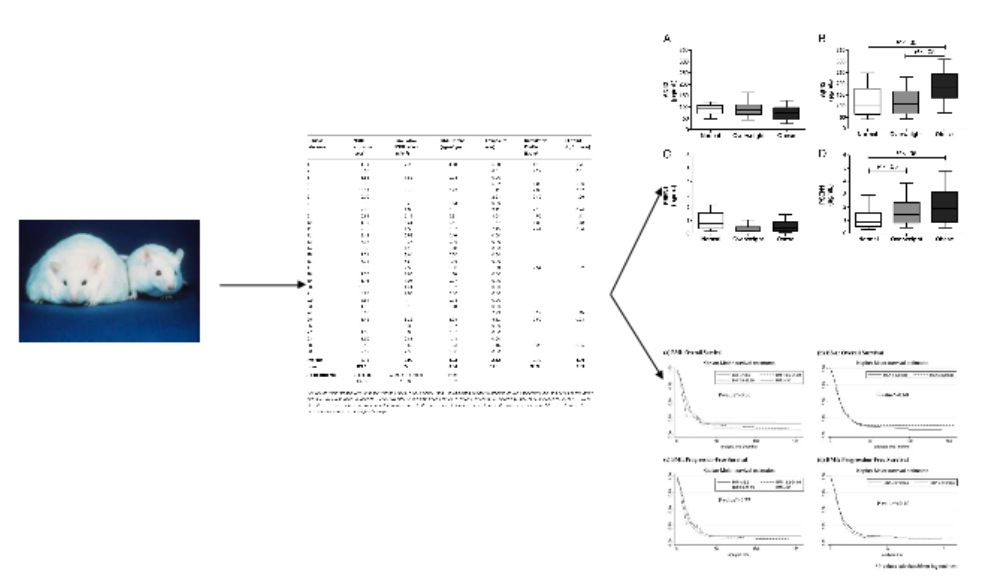
\includegraphics[width=100mm]{images/diseaseStudyClassic.png}
	\end{figure} 
\end{frame}



\begin{frame}
	\frametitle{Single-omics analysis: The first decade of the XXIst}
	\begin{figure}[ht]
		\centering
		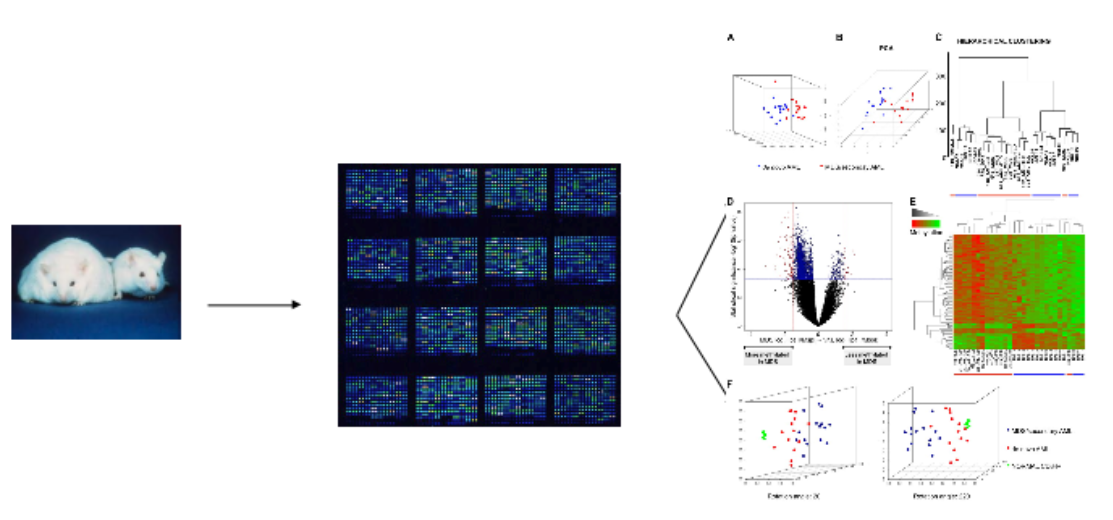
\includegraphics[width=100mm]{images/diseaseStudySingleOmics.png}
	\end{figure} 
\end{frame}



%\begin{frame}
%	\frametitle{Today: Multi-omics studies have become normal }
%	\begin{figure}[ht]
%		\centering
%		\includegraphics[width=100mm]{images/multiOmicsDatasets.png}
%	\end{figure} 
%\end{frame}
 
\subsection{Why should we integrate data?}
  
  
  \begin{frame}
  	\frametitle{Why should we integrate data?}
  	The Blind Men and the Elephant
  	\begin{figure}[ht]
  		\centering
  		\includegraphics[width=50mm]{images/Captura1.PNG}
  	\end{figure} 
  \textbf{	What we learn from an experiment may depend on where we look, how we look, and the scope of our view!}
  {\tiny 	\url{http://www.noogenesis.com/pineapple/blind_men_elephant.html }}
  \end{frame}
  
  
  \begin{frame}
  	\frametitle{Focussing only on one platform risks missing an obvious signal}
  		\begin{figure}[ht]
  			\centering
  			\includegraphics[width=100mm]{images/Imagen22.jpg}
  		\end{figure} 
  \end{frame}
  
  
  \begin{frame}
  	\frametitle{So let's measure as many as possible}
  		\begin{figure}[ht]
  			\centering
  			\includegraphics[width=100mm]{images/Captura2.PNG}
  		\end{figure} 
  \end{frame}
  
  
  
  \begin{frame}
  	\frametitle{From componentwise to global approaches}
  	\begin{columns}%
  		
  		\begin{column}[t]{0.45\textwidth}%
  			\begin{figure}[ht]
  				\centering
  				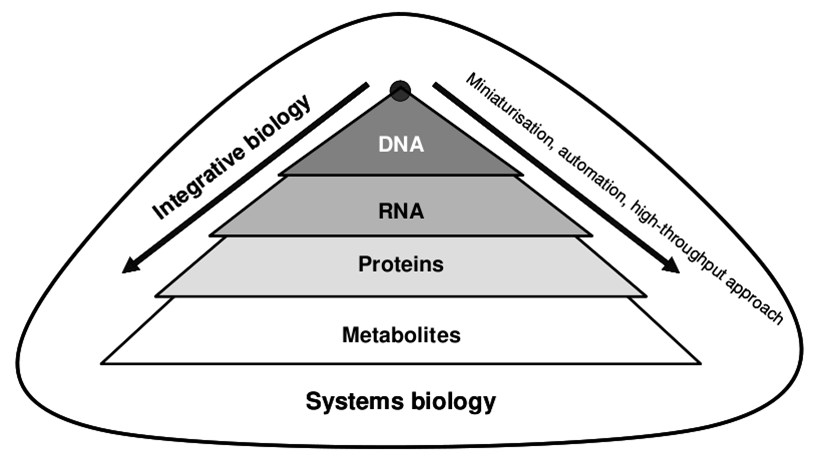
\includegraphics[width=50mm]{images/Imagen24.png}
  			\end{figure} 
  		\end{column}
  		
  		\begin{column}[t]{0.45\textwidth}%
  			\begin{itemize}
  				\item It is expected that the integrated collection and analysis of diverse types of data,
  				\item jointly modelled and analyzed in a systems biology approach 
  				\item can shed light on the global functioning of biological systems.
  			\end{itemize}
  		\end{column}
  		
  	\end{columns}
  \end{frame} 
  

\begin{frame}
  	\frametitle{Ultimate Goal (1): understanding of complex processes
  		}
  		\begin{figure}[ht]
  			\centering
  			\includegraphics[width=90mm]{images/imagen25.png}
  		\end{figure} 
\end{frame}
  
  
   \begin{frame}
   	\frametitle{Ultimate Goal (2): Improved Robust Biomarkers}
   	\begin{figure}[ht]
   		\centering
   		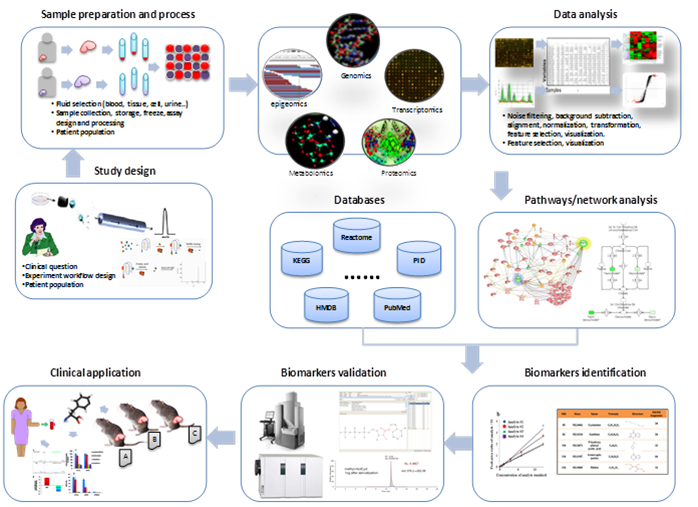
\includegraphics[height=0.8\textheight]{images/Imagen26.png}
   	\end{figure} 
   \end{frame}
  
 
 %\subsection{Integrative Analysis and Data integration: methods, types, tools, challenges}
  
%  \begin{frame}
%  	\frametitle{Data Integration is cool}
%  	\begin{itemize}
%  		\item Everywhere nowadays in Biology, Medicine, Bioinformatics, [BTW much less in Statistics]
%  		\begin{itemize}
%  			\item Meetings: Barcelona (Feb. 2013), Leiden (Apr. 2013), Ascona (May 2013), Crete (Nov 2014) and many more
%  			\item Financing (FP7): projects with $> 10^6 €$ each (Stategra,	MimOmics).
%  			\item Increasing use of 'data integration' in publication titles.
%  		\end{itemize}
%  	\end{itemize}
%  		\begin{figure}[ht]
%  			\centering
%  			\includegraphics[width=30mm]{images/Imagen27.png}
%  		\end{figure} 
% \end{frame}
  
  
  \begin{frame}
  	\frametitle{But what is Data Integration?}
  	\begin{itemize}
  		\item ``\textit{Data integration}'' may mean different things...
  		\begin{itemize}
  			\item Computational combination of data 
  			\item Combination of studies performed independently
  			\item Simultaneous analysis of multiple variables on multiple datasets.
  			\item Not to mention any possible approach for homogeneously querying heterogeneous data sources
  		\end{itemize}
  		\item \textbf{Integrative analysis} may be preferable
  	\end{itemize}
  \end{frame}
 
 \section{Methods and Tools for IODA}
 
 \begin{frame}
 	\begin{center}
 		{\huge 	Methods and Tools for IODA}
 	\end{center}
 \end{frame}
 
  
  \begin{frame}
  	\frametitle{Integrative Omics Data Analysis}
  	\begin{itemize}
  		\item The idea that efficient integration of data from different OMICS can greatly facilitate the discovery of true causes and states of disease is rapidly pervading the biomedical community
  		\item The aims of integrative analysis is the deciphering of complex biological relationships empowered by the combined use of distinct pieces of information that represent a, probably partial, view of the different levels at which these processes happen
  	\end{itemize}
  \end{frame}
  
  
   \begin{frame}
   	\frametitle{There are many types of integrative analysis}
   		\begin{figure}[ht]
   			\centering
   			\includegraphics[height=0.8\textheight]{images/Imagen28.jpg}
   			\caption{Hamid et al. 2009}
   		\end{figure} 
   \end{frame}
   
   
   \begin{frame}
   	\frametitle{There are many methods ...}
\vspace{-0.5cm}
   		\begin{figure}[ht]
   			\centering
   			\includegraphics[width=0.7\textwidth]{images/IODAmethods2020.png}
%   				\caption{}}
   		\end{figure} 
\vspace{-0.5cm}   	{\tiny Subramanian et alt., 2020. \textit{Multi-omics Data Integration, Interpretation, and Its Application}}
   \end{frame}
  
  
   \begin{frame}
   	\frametitle{There are many data repositories}
 \vspace{-1 cm}
   	\begin{figure}[ht]
   		\centering
   		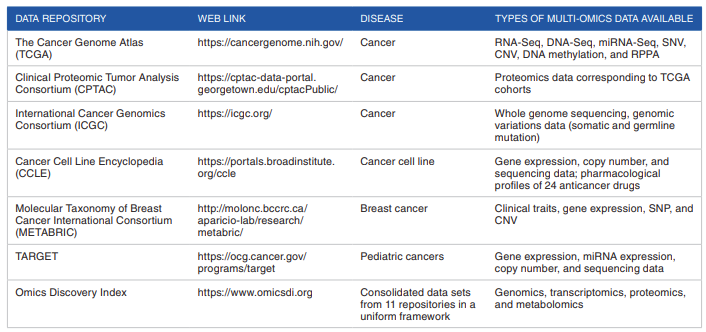
\includegraphics[height=0.7\textheight]{images/IODADataRepositories2020.png}
   	\end{figure}
\vspace{-0.5cm}   	{\tiny Subramanian et alt., 2020. \textit{Multi-omics Data Integration, Interpretation, and Its Application}}
   \end{frame}
   
   
\begin{frame}
    	\frametitle{And many Data Visualization Portals}
 \vspace{-0.25 cm}
    	\begin{figure}[ht]
    		\centering
    		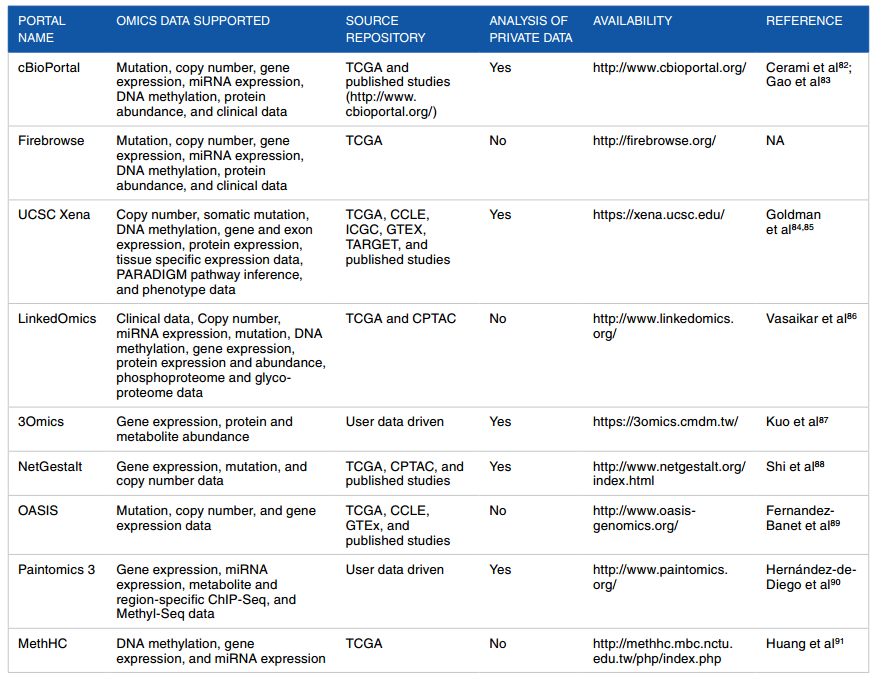
\includegraphics[width=90mm]{images/IODAVisualizationPortals.png}
    	\end{figure} 
%\vspace{-0.5cm}   	{\tiny Subramanian et alt., 2020. \textit{Multi-omics Data Integration, Interpretation, and Its Application}}
\end{frame} 
    

 \frame{
  	\frametitle{So what?}
  	\begin{itemize}
  		\item We willl restrict to arbitrarily chosen situation
  		\begin{itemize}
  			\item Multivariate statistical methods, classic and extensions
  		\end{itemize}
  		\item for which we will sketch basic ideas, 
  		\begin{itemize}
  			\item General concept
  			\item Basic formulation
  		\end{itemize}
  		\item and provide some examples of use
  	\end{itemize}
  }


\subsection {An overview of analysis methods}

\subsection{Multivariate Statistical Methods}

\begin{frame}
	\frametitle{Multivariate statistics in genomics}
	\begin{columns}%
		
		\begin{column}[t]{0.65\textwidth}%
			\begin{itemize}
				\item Multivariate methods have pervaded the field of genomics since its very beginning
				\begin{itemize}
					\item The (in)fammous clustering (HC, heatmaps)
					\item Matriz factorizations / Dimension reduction (PCA, SVD, CoA )
					\item Discriminant Analyses (LDA $->$ DLDA, ...)
				\end{itemize}
			\end{itemize}
			To cite but a few.
		\end{column}
		
		\begin{column}[t]{0.25\textwidth}%
			\begin{figure}[ht]
				\centering
				\includegraphics[width=35mm]{images/Captura7.PNG}
			\end{figure} 
		\end{column}
	\end{columns}
\end{frame} 

\begin{frame}
	\frametitle{Best approach for omics data analysis?}
	\begin{columns}%
		
		\begin{column}[t]{0.40\textwidth}%
			\begin{itemize}
				\item Classical Statistics
				\begin{itemize}
					\item Multiple regression
					\item Discriminant analysis 
					\item ANOVA
				\end{itemize}
				\item Data tables are long and lean
			\end{itemize}
		\end{column}
		
		\begin{column}[t]{0.15\textwidth}%
			\begin{figure}[ht]
				\centering
				\includegraphics[width=15mm]{images/Imagen32.png}
			\end{figure}   			
		\end{column}
		\begin{column}[t]{0.4\textwidth}%
			\begin{itemize}
				\item Assumptions
				\begin{itemize}
					\item Independent variables
					\item More observations than variables
					\item Multivariate normality
					\item Interested in one dependent
					\item Few missings
				\end{itemize}
				\item DO NOT hold for many omics data 
			\end{itemize}
		\end{column}
	\end{columns}
\end{frame} 

\begin{frame}
	\frametitle{The nature of omics data}
	\begin{itemize}
		\item Omics data are diverse
		\begin{itemize}
			\item They measure distinct characteristics
			\begin{itemize}
				\item GC/MS spectrum, Expression, Concentration…
			\end{itemize}
		\end{itemize}
		\item Although they have aspects in common
		\begin{itemize}
			\item Most of them are high throughput
			\begin{itemize}
				\item Many variables (K) measured simultaneously
			\end{itemize}
			\item Relatively expensive, ethical limitations, regulations
			\begin{itemize}
				\item Few samples (N) analyzed 
			\end{itemize}
		\end{itemize}
	\end{itemize}
	%\hspace{4cm}$K >> N$
	\begin{figure}[ht]
		\centering
		\includegraphics[width=40mm]{images/Imagen31.png}
		\caption{$K >> N$}
	\end{figure} 
\end{frame}

\begin{frame}
	\frametitle{A Better Way}
	\begin{itemize}
		\item Multivariate analysis by projection (dimension-reduction, matrix decomposition) methods
		\begin{itemize}
			\item Looks at ALL the variables together
			\item Avoids loss of information
			\item Finds underlying trends = ``latent variables''
			\item More stable models
		\end{itemize}
	\end{itemize}
	\begin{figure}[ht]
		\centering
		\includegraphics[width=65mm]{images/Imagen33.png}
	\end{figure}
\end{frame}


\frame<0>{
	\frametitle{A not-so random walk by classical MVA}
	\begin{itemize}
		\item ``Classical multivariate statistical methods'' (whatever this means) have been thoroughly used in the analysis of omics data.
		\item We review some methods and applications
		\begin{itemize}
			\item Principal components analysis (PCA)
			\item Singular value decomposition (SVD)
			\item Correspondence analysis (CoA)
			\item Factor analysis (FA)
		\end{itemize}
	\end{itemize}
}

\subsection{From PCA to Multiple Factor Analysis}

\begin{frame}
	\frametitle{Principal Components Analysis}
	\begin{itemize}
		\item PCA is an statistical method that can be traced back to Pearson (1901) or Hotelling (1933).
		\item Its main goals are
		\begin{itemize}
			\item Capture the information provided by the original variables using a smaller number of new variables
			\item Provide a representation of the data in reduced dimension
		\end{itemize}
		\item PCA is intimately related with the most famous \texttt{Matrix Factorization} method.
	\end{itemize}
\end{frame}



\begin{frame}
	\frametitle{What does PCA do? }
	\begin{itemize}
		\item Given a $k\times n$ data matrix containing $k$ (probably correlated) measurements on n samples (objects/individuals...), PCA decomposes this matrix in new $k$ components such that they
		\begin{itemize}
			\item account for different sources of variability in the data,
			\item are uncorrelated, that is each component accounts for a different source of variability,
			\item have decreasing explanatory ability: each component explains more than the following
			\item allow for a lower dimensional representation of the data in terms of scores on principal components.
			\item get an overview of the dominant patterns and major trends in the data (visualize clusters, identify outliers)
		\end{itemize}
	\end{itemize}
\end{frame}


\begin{frame}
	\frametitle{PCA is an example of \textit{Matrix Factorization}}
\vspace{-0.25 cm}
\begin{figure}[ht]
	\centering
	\includegraphics[width=60mm]{images/matrixFactorization1.jpg}
\end{figure} 
\vspace{-0.5cm}   	{\tiny Stein-O'Brian et alt., 2017. \textit{Enter the Matrix: Factorization Uncovers Knowledge from Omics
}}
\end{frame}

\begin{frame}
	\frametitle{Matrix Product of Amplitude $\times$ Pattern Matrices} \framesubtitle{An Approximation the Preprocessed Input Data Matrix  }
	\vspace{-0.25 cm}
	\begin{figure}[ht]
		\centering
		\includegraphics[width=60mm]{images/matrixFactorization2.jpg}
	\end{figure} 
	\vspace{-0.5cm}   	{\tiny Stein-O'Brian et alt., 2017. \textit{Enter the Matrix: Factorization Uncovers Knowledge from Omics
	}}
\end{frame}


\begin{frame}
	\frametitle{MFs provide data visualization in \textit{reduced dimension}}
	\begin{figure}[ht]
		\centering
		\includegraphics[width=100mm]{images/Imagen34.png}
	\end{figure}
\end{frame}


\begin{frame}
	\frametitle{Applications of PCA}
	\begin{itemize}
		\item PCA has been used in a wealth of applications 
		\item The best known 
		\begin{itemize}
			\item Batch effect detection
			\item Pattern recognition
		\end{itemize}
		\item Besides standard applications there exist many extensions
		\begin{itemize}
			\item Probabilistic PCA, Bayesian PCA, Inverse non-linear PCA, Nipals PCA, Robust PCA
		\end{itemize}
	\end{itemize}
\end{frame}



\begin{frame}
	\frametitle{Examples}
	\begin{figure}[ht]
		\centering
		\includegraphics[width=100mm]{images/Captura8.PNG}
	\end{figure}
\end{frame}


\begin{frame}
	\frametitle{Examples}
	\begin{figure}[ht]
		\centering
		\includegraphics[width=100mm]{images/Captura9.PNG}
	\end{figure}
\end{frame}

\begin{frame}
	\frametitle{When single matrix factorization is not enough}
	\begin{itemize}
		\item Ideally matrix factorizations can proide dimension-reduced data visualizations that help detect distinct patterns in features or samples.
		\item Sometimes the information in the data does not allow for this separation, but extending the factorization to \textbf{different omics} that can be \textit{related differently} with the latent factors can do the job.
		\item As could be expected there exist many ways to do multiple factorization.
		\begin{itemize}
			\item Multiple Factor Analysis, Regularized Generalized Canonical Correlation Analysis, Multiple Coinertia Analysis, ...
		\end{itemize}
	\end{itemize}
\end{frame}

\begin{frame}
	\frametitle{Example: Multi-omics analysis of colorectal cancer data}
	\framesubtitle{Integrative Analysis of Expression, Mutations and Copy Number Variation}
	
	\begin{itemize}
		\item A set of 121 tumors from the TCGA (Weinstein, Collisson, Mills, et al. 2013) colorectal cancer cohort is analyzed. 
		\item The tumors have been profiled for 
			\begin{itemize} 
				\item gene expression using RNA-seq, 
				\item mutations using Exome-seq, and 
				\item copy number variations using genotyping arrays. 
			\end{itemize}
		\item Although two tumors arise in the colon, they may have distinct \textit{molecular profiles}, which is important for treatment decisions. 
		\item The subset of tumors used in this chapter belong to two distinct molecular subtypes CMS1, CMS3
	\end{itemize}
	
\end{frame}
	
\begin{frame}
	\frametitle{Example: Multi-omics analysis of colorectal cancer data}
	\framesubtitle{Expression, Mutations and Copy Number Variation data}	
	\begin{figure}[ht]
		\centering
		\includegraphics[width=100mm]{images/dataMultiomicsColonCancerStudy.png}
	\end{figure}
\end{frame}
	
\begin{frame}
	\frametitle{Example: Multi-omics analysis of colorectal cancer data}
	\framesubtitle{Individual omics do not separate well tumor types}	
	\begin{figure}[ht]
		\centering
		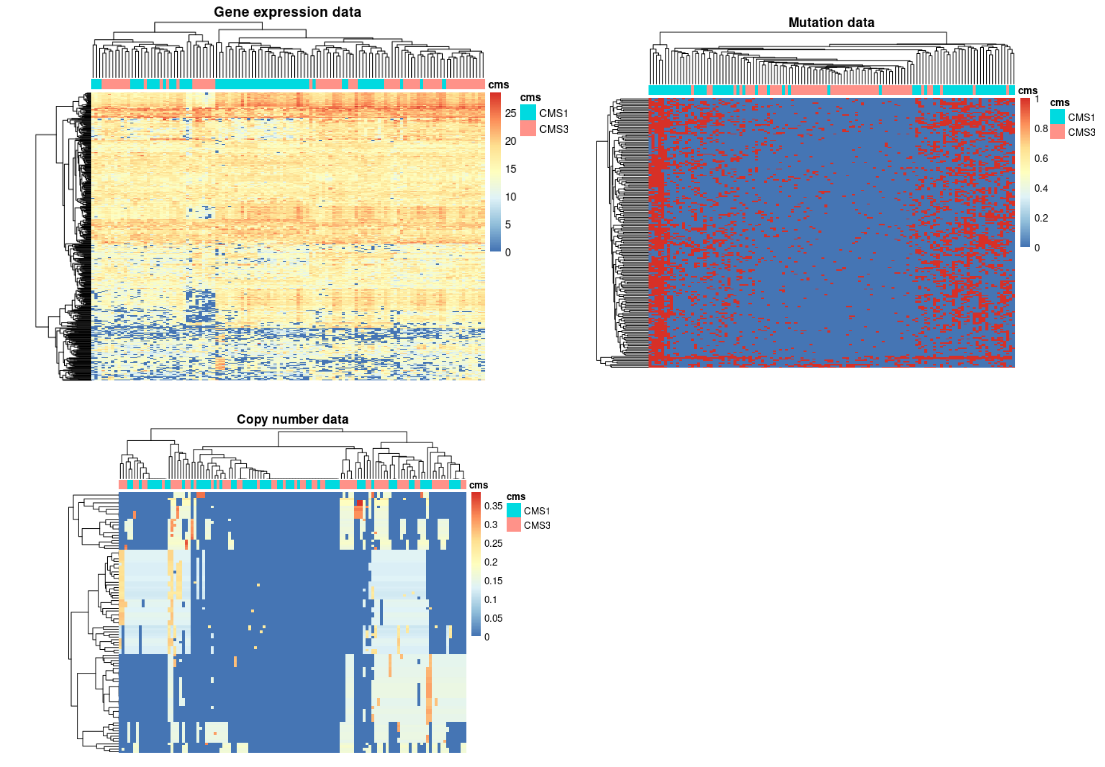
\includegraphics[width=100mm]{images/heatmapsMultiomicsColonCancerStudy1.png}
	\end{figure}
\end{frame}

\begin{frame}
	\frametitle{Multiple Factor Analysis}
	\framesubtitle{An extension of PCA to multiple data tables}
	\begin{center}
		\includegraphics[height=0.7\textheight]{images/multipleFactorAnalysis.png}
	\end{center}

    {\center \large \url{http://factominer.free.fr}}
\end{frame}

\begin{frame}
	\frametitle{Example: Multi-omics analysis of colorectal cancer data}
	\framesubtitle{Joint omics factorization provides much better separation}	
	\begin{figure}[ht]
		\centering
		\includegraphics[width=100mm]{images/multipleFactorAnalysisInColonCancer.png}
	\end{figure}
\end{frame}



\begin{frame}
	\frametitle{Are there alternatives?}
	\framesubtitle{There are many -or too many- alternative approaches}
	\begin{center}
		\includegraphics[height=0.7\textheight]{images/awesomeMultiOmics.png}
	\end{center}
    {\center \large \url{https://github.com/mikelove/awesome-multi-omics}}
\end{frame}


%\begin{frame}
%	\frametitle{MixOmics: Integrative Analysis of Multiple Omics Data with Sparse Multivariate Methods}
%	\begin{center}
%		\includegraphics[height=0.7\textheight]{images/mixOmics1.png}
%	\end{center}
%\end{frame}

\section{In summary, the lights and the shadows}

\frame[allowframebreaks]{
\frametitle{Summary}
\begin{itemize}

	\item There is no universal ``IODA'' method 
	\item Many families of many types of methods available: 
	Need to be related, classified, filtered, benchmarked.
   \begin{itemize}
		\item In many situations biology must guide the analysis
		\item For example, miRNAs-mRNAs or mRNAS-Methylation
	\end{itemize}
   \begin{itemize}
	\item All data are not equally informative.
	\item It is often the case that some omics dominate others
	\item Gene expression and what else?
\end{itemize}

\framebreak

	\item Promising approaches are those that
	\begin{itemize}
		\item Allow inclusion of biological information,
		\item Provide hints for interpretability
		\item Implementations are available
		\item E.g. See the MOFA package
	\end{itemize}

	\item Biological question should be first.

	\item There are more mathematical/statistical tools than end-user bioinformatical solutions: Opportunity for developers
	
	\item Nothing said about ML/DL but clearly helpful in many situations.
	
\end{itemize}
}

\begin{frame}
	\frametitle{Acknowledgements}
	\begin{center}
		\includegraphics[height=0.7\textheight]{images/acknowledgements.png}
	\end{center}
\end{frame}


\end{document}

\section{Examples and case studies}

\frame[allowframebreaks]{
	\frametitle{Integrative Analysis of Expression and Methylation}
	\begin{itemize}
		\item Methylation of CpG dinucleotides in the promoter of genes
		involved in the oncogenic process has been shown to be a key process
		contributing to tumor initiation and/or progression.
		\item Essentially (and especially in cancer) methylation acts by inhibiting gene expression that
		is,\emph{ the more methylated is a gene the more repressed is its expression}
	\end{itemize}
	
	\begin{center}
		\includegraphics[width=\textwidth]{./images/methylationAction1.png}
	\end{center}
	
	\begin{center}
		\includegraphics[width=0.9\textwidth]{./images/methSitesVSexprSites.png}
	\end{center}
	
	\begin{itemize}
		\item Although the relation between methylation and gene expression is probably continuous ("\emph{the more...the less...}"),
		\begin{center}
			\includegraphics[width=0.7\textwidth]{./images/DNA-Methylation-and-Gene-Expression-Relationship.jpg}
		\end{center}
		\item methylation is, in practice, seen as a dual phenomenon
		\begin{itemize}
			\item A methylated gene is ``off''
			\item An unmethylated gene is ``on''
		\end{itemize}
		\item Practical problem: \textbf{\emph{at which methylation level a gene is seen as ``methylated'' (is it ``turned off'')?}}
	\end{itemize}
	
	\framebreak
	
	\begin{itemize}
		\item Considering the relation between methylation and expression in cancer (the higher methylation the lower the expression...)
		\item leads to expecting that scatterplots depicting the relation between methylation and expression show a negative correlation.
		\item This is so and indeed genes known to be regulated by methylation use to show an L-shape pattern in these plots.
	\end{itemize}
	\begin{center}
		\includegraphics[width=0.7\textwidth]{./images/Lshapes1.png}
	\end{center}
	
	\framebreak
	
	\emph{Integrative analysis of methylation and gene expression data in TCGA} (Liu\& Qiu, 2012)
	\begin{center}
		\includegraphics[width=0.75\textwidth]{images/L-shape1.png}
	\end{center}
	
}	



\frame[allowframebreaks]{
	\frametitle{Integrative Analysis of mRNA and miRNA}
	
	\begin{enumerate}
		\item miRNAs are small RNA molecules that are key regulators of the expression of certain genes
		\item These genes are called their mRNA targets.
		\item Only one-of-several transcription--regulating mechanisms. Others mechanisms: Alternative splicing, polyadenilation.
		\item Although there are exceptions the general statement is that miRNAs act to repress the expression of their targets.
	\end{enumerate}
	
	\begin{center}
		\includegraphics[width=0.9\textwidth]{./images/microRNAs0.jpg}
	\end{center}	
	
	\framebreak
	
	Every mRNA may target many genes, \\
	Any gene may be the target of many miRNAs
	
	\begin{center}
		\includegraphics[width=0.7\textwidth]{./images/n2nMicroRNAs.png}
	\end{center}	
	
	\begin{center}
		\includegraphics[width=0.9\textwidth]{./images/microRNAMethods.png}
	\end{center}
	
	\begin{center}
		\includegraphics[width=0.9\textwidth]{./images/microRNATools.png}
	\end{center}	
	\framebreak
	\begin{center}
		\includegraphics[width=0.9\textwidth]{./images/miRNAresults1.png}
	\end{center}	
}	

\frame[allowframebreaks]{
	\frametitle{Integrating clinical and Omics data}
	\begin{center}
		\includegraphics[width=0.7\textwidth]{./images/translationalPlatforms.png}
	\end{center}	
	
	\begin{center}
		\includegraphics[width=0.9\textwidth]{./images/cBioPortal.png}
	\end{center}	
	
}	
